\documentclass[12pt, a4paper]{article}
\usepackage[utf8]{inputenc}
\usepackage{geometry}
\geometry{a4paper, margin=1in}
\usepackage{graphicx}
\usepackage{hyperref}
\usepackage{listings}
\usepackage{xcolor}
\usepackage{booktabs}

% Custom Colors for code listing
\definecolor{codegreen}{rgb}{0,0.6,0}
\definecolor{codegray}{rgb}{0.5,0.5,0.5}
\definecolor{codepurple}{rgb}{0.58,0,0.82}
\definecolor{backcolour}{rgb}{0.95,0.95,0.92}

\lstdefinestyle{mystyle}{
    backgroundcolor=\color{backcolour},   
    commentstyle=\color{codegreen},
    keywordstyle=\color{magenta},
    numberstyle=\tiny\color{codegray},
    stringstyle=\color{codepurple},
    basicstyle=\ttfamily\footnotesize,
    breakatwhitespace=false,         
    breaklines=true,                 
    captionpos=b,                    
    keepspaces=true,                 
    numbers=left,                    
    numbersep=5pt,                  
    showspaces=false,                
    showstringspaces=false,
    showtabs=false,                  
    tabsize=2
}
\lstset{style=mystyle}



\title{\textbf{23CSE352: Big Data Analytics}\\ \Large Project Review 1 Report \\ \vspace{0.5cm} \Large \textbf{Big Data Analytics of Crime Patterns using Hadoop MapReduce and Apache Hive}}
\author{Group Members:\\ \textit{(Add Your Names Here)}}
\date{\today}

\begin{document}

\maketitle
\tableofcontents
\newpage

\section{Introduction}
This project aims to process and analyze crime data from the City of Chicago using Big Data technologies. With millions of records detailing various aspects of crime occurrences, this data requires distributed processing tools like Hadoop MapReduce and Apache Hive. By leveraging these frameworks, we extract meaningful insights, such as frequency of crime types, high-crime areas, and historical trends, transforming raw data into actionable intelligence.

\section{Problem Statement}
Law enforcement agencies and city planners require accurate and fast analysis of crime records to optimize resource allocation and enhance public safety. Processing large-scale crime datasets using traditional sequential systems is inefficient and time-consuming. The problem addressed in this project is to implement a scalable pipeline that efficiently counts crime frequencies and performs complex SQL-like analytics on a large real-world dataset.

\section{Motivation}
The motivation for this project stems from the critical need for data-driven decision-making in public safety. Analyzing crime patterns helps in understanding the socio-economic impact of crimes and assists police departments in predictive policing and strategic deployment. Utilizing Big Data technologies ensures that the analysis can scale with continuously growing datasets.

\section{Dataset}
\textbf{Name:} Chicago Crimes (2001 to Present)\\
\textbf{Source:} \url{https://data.cityofchicago.org/Public-Safety/Crimes-2001-to-Present/ijzp-q8t2}\\
\textbf{Description:} A comprehensive real-world dataset containing incident reports of crimes occurred in the City of Chicago. We have fetched a subset of 10,000 recent records via the official API to satisfy the project constraints. The key attributes are summarized below:

\begin{table}[h]
    \centering
    \begin{tabular}{@{}ll@{}}
        \toprule
        \textbf{Attribute Category} & \textbf{Fields} \\ \midrule
        Identifiers & \texttt{id}, \texttt{case\_number}, \texttt{date} \\
        Crime Typology & \texttt{primary\_type}, \texttt{description} \\
        Location Data & \texttt{location\_description}, \texttt{district}, \texttt{ward}, \texttt{community\_area} \\
        Boolean Flags & \texttt{arrest}, \texttt{domestic} \\ \bottomrule
    \end{tabular}
    \caption{Dataset Attributes Overview}
\end{table}

\section{Architecture}
The project follows a standard Big Data processing pipeline:
\begin{enumerate}
    \item \textbf{Data Ingestion:} The dataset is downloaded as a CSV file, cleaned to remove embedded newlines, and uploaded to the Hadoop Distributed File System (HDFS).
    \item \textbf{MapReduce Processing:} A Java-based MapReduce job is executed on Hadoop to parse the data in parallel and aggregate crime counts.
    \item \textbf{Hive Analytics:} The dataset is loaded into Apache Hive with an \texttt{OpenCSVSerde}. 10 complex queries are executed to perform advanced data summarization.
\end{enumerate}

\section{MapReduce Problem}
The MapReduce problem we are solving is \textbf{Category-wise Statistics}: determining the frequency of each primary crime type (e.g., THEFT, BATTERY) across the entire dataset.

\section{Mapper logic explanation}
The Mapper takes a line of the CSV file as input. It skips the header row. It then splits the line using a regular expression that correctly handles commas inside double quotes. The \texttt{primary\_type} attribute is extracted from the 6th column, cleaned of quotes, and emitted as the intermediate key with a value of 1.

\section{MapReduce source code}
Below is the Java MapReduce code containing the Mapper (and Driver) classes:
\begin{lstlisting}[language=Java]
package bigdata;

import java.io.IOException;
import org.apache.hadoop.conf.Configuration;
import org.apache.hadoop.fs.Path;
import org.apache.hadoop.io.IntWritable;
import org.apache.hadoop.io.Text;
import org.apache.hadoop.mapreduce.Job;
import org.apache.hadoop.mapreduce.Mapper;
import org.apache.hadoop.mapreduce.Reducer;
import org.apache.hadoop.mapreduce.lib.input.FileInputFormat;
import org.apache.hadoop.mapreduce.lib.output.FileOutputFormat;

public class CrimeTypeCount {

    public static class CrimeMapper extends Mapper<Object, Text, Text, IntWritable> {
        private final static IntWritable one = new IntWritable(1);
        private Text crimeType = new Text();

        public void map(Object key, Text value, Context context) throws IOException, InterruptedException {
            String line = value.toString();
            if (line.startsWith("\"id\"")) return; // Skip header

            String[] fields = line.split(",(?=(?:[^\"]*\"[^\"]*\")*[^\"]*$)");
            if (fields.length > 5) {
                String type = fields[5].replaceAll("^\"|\"$", "").trim();
                if (!type.isEmpty()) {
                    crimeType.set(type);
                    context.write(crimeType, one);
                }
            }
        }
    }
}
\end{lstlisting}

\section{Reducer Logic}
The Reducer receives the intermediate key (\texttt{primary\_type}) and an iterable list of values (mostly 1s) emitted by the Mappers. It iterates through these values, summing them up to calculate the total frequency of each crime type, and emits the final result as \texttt{(CrimeType, TotalCount)}.

\section{Reducer code}
\begin{lstlisting}[language=Java]
    public static class CrimeReducer extends Reducer<Text, IntWritable, Text, IntWritable> {
        private IntWritable result = new IntWritable();

        public void reduce(Text key, Iterable<IntWritable> values, Context context) throws IOException, InterruptedException {
            int sum = 0;
            for (IntWritable val : values) {
                sum += val.get();
            }
            result.set(sum);
            context.write(key, result);
        }
    }
\end{lstlisting}

\section{Input and Output}
\textbf{Input:} A cleaned CSV file residing in HDFS at \texttt{/user/\$USER/bigdata\_project/crimes/chicago\_crimes\_clean.csv}. \\
\textbf{Output:} A text file generated by Hadoop in \texttt{/user/\$USER/bigdata\_project/crime\_output/} containing lines of tab-separated crime types and their total counts (e.g., \texttt{THEFT  2150}).

\section{Screenshots of execution}
\textit{(Replace the placeholder images with your actual screenshots)}

\subsection{HDFS Storage}
\begin{figure}[h]
    \centering
    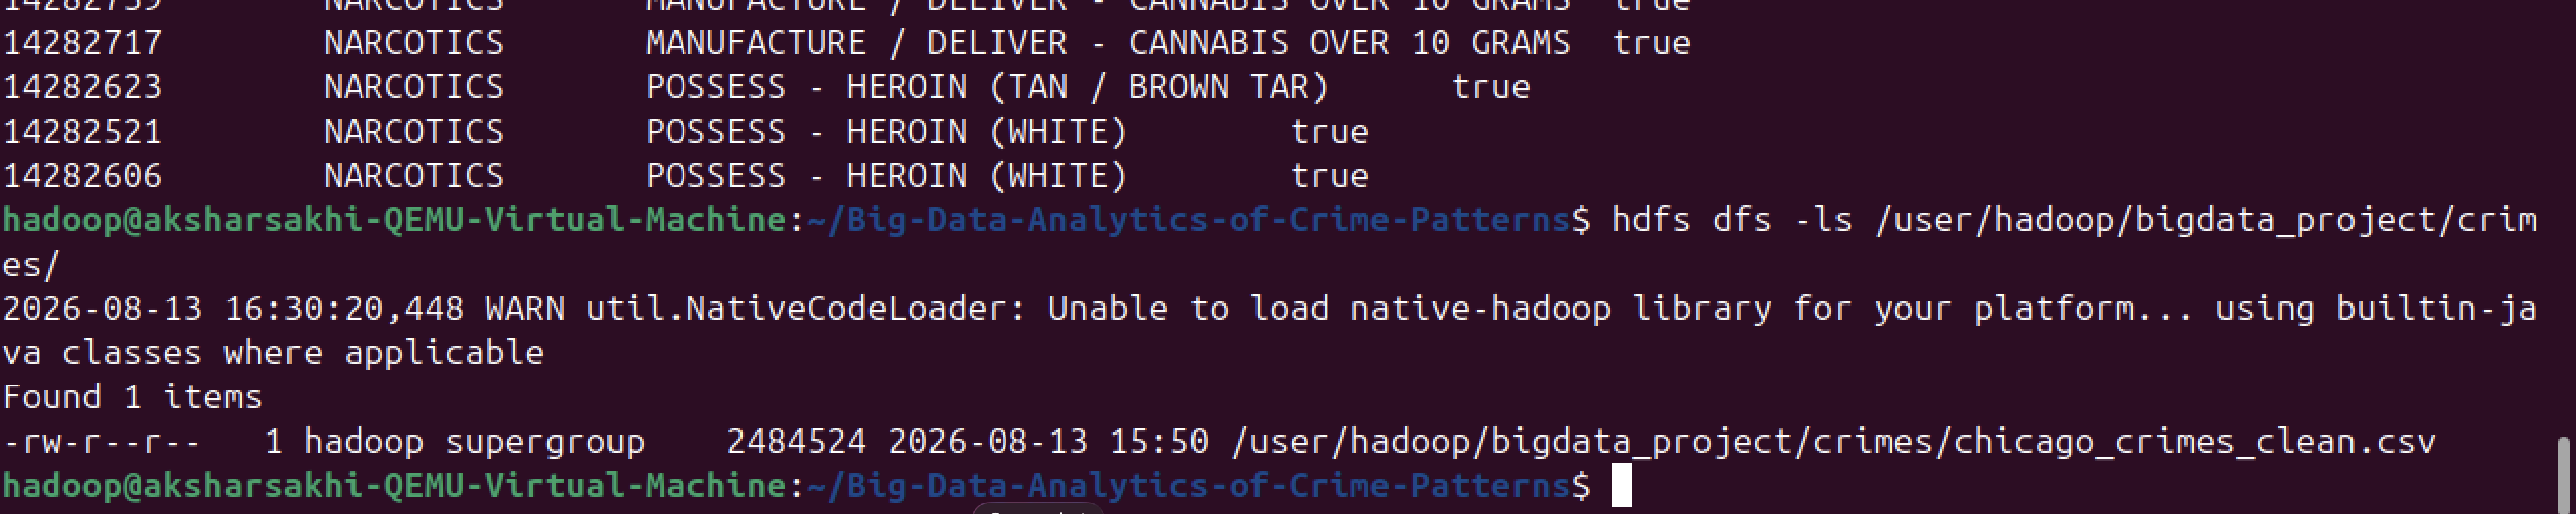
\includegraphics[width=0.8\textwidth]{images/hdfs_screenshot.png}
    \caption{Uploading dataset to HDFS and verifying storage.}
\end{figure}

\subsection{MapReduce Execution}
\begin{figure}[h]
    \centering
    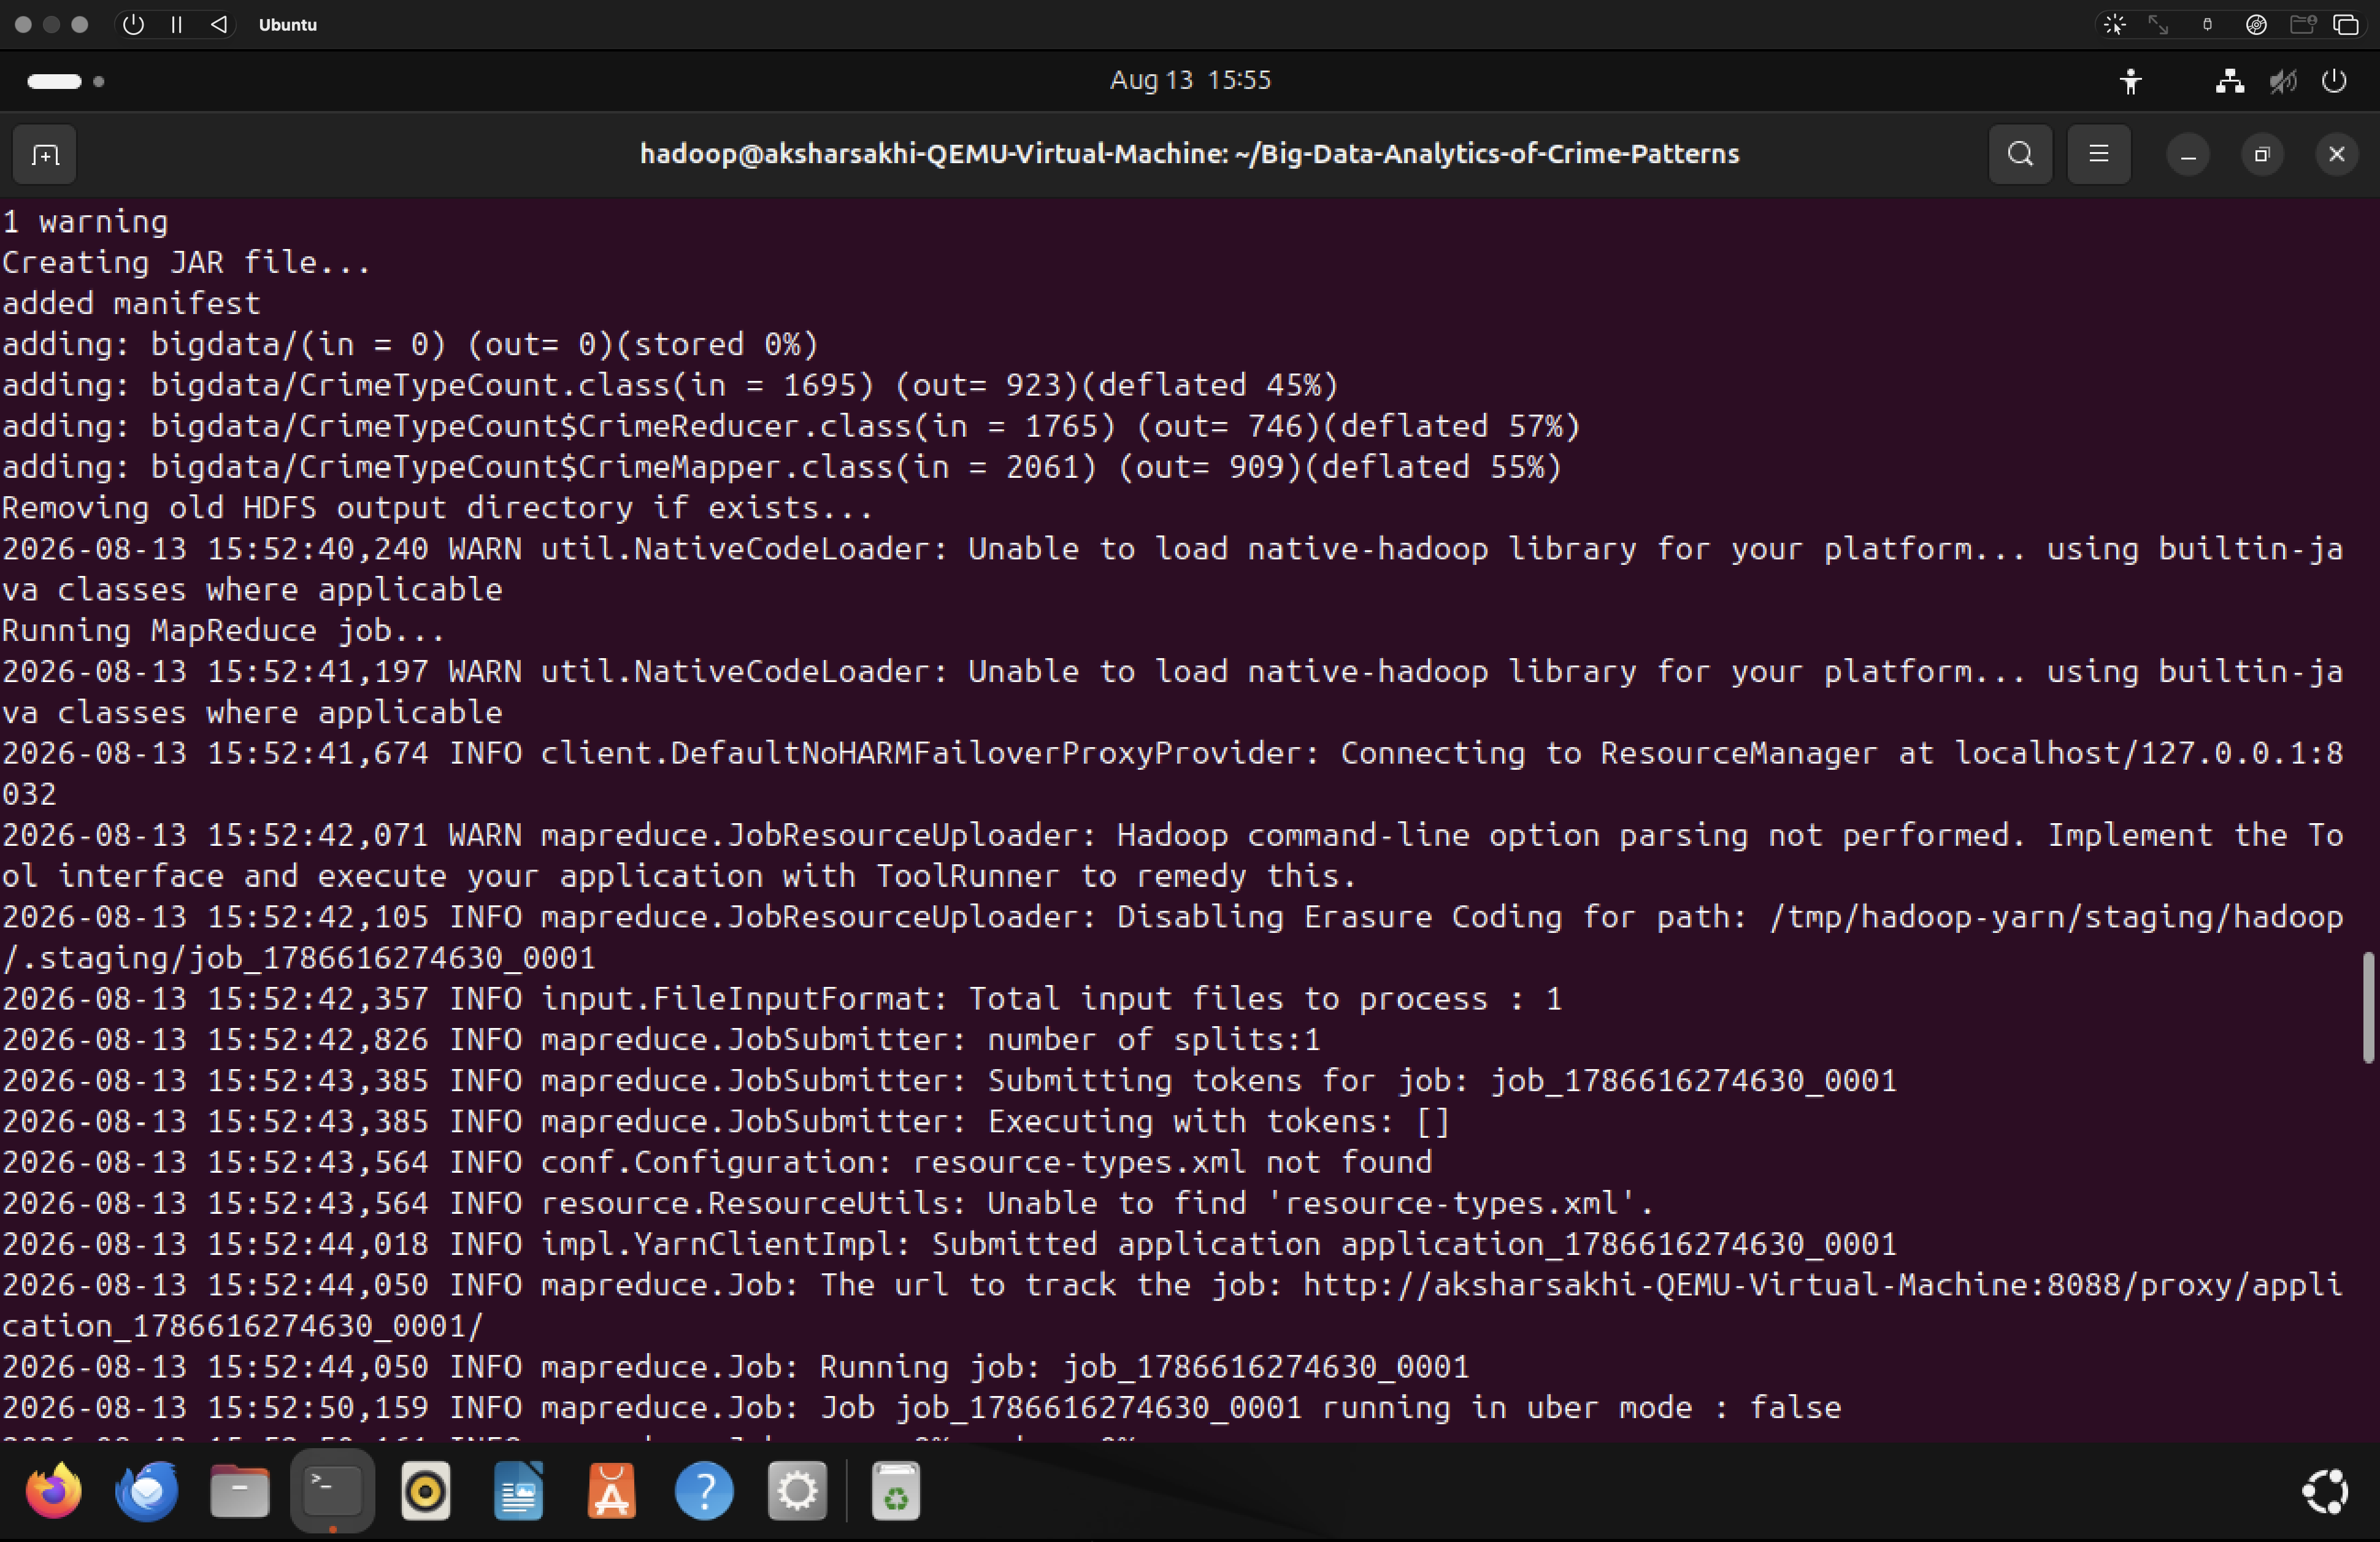
\includegraphics[width=0.8\textwidth]{images/mr_execution.png}
    \caption{Executing the MapReduce Job on the Hadoop Cluster.}
\end{figure}

\section{Output screenshots}
\begin{figure}[h]
    \centering
    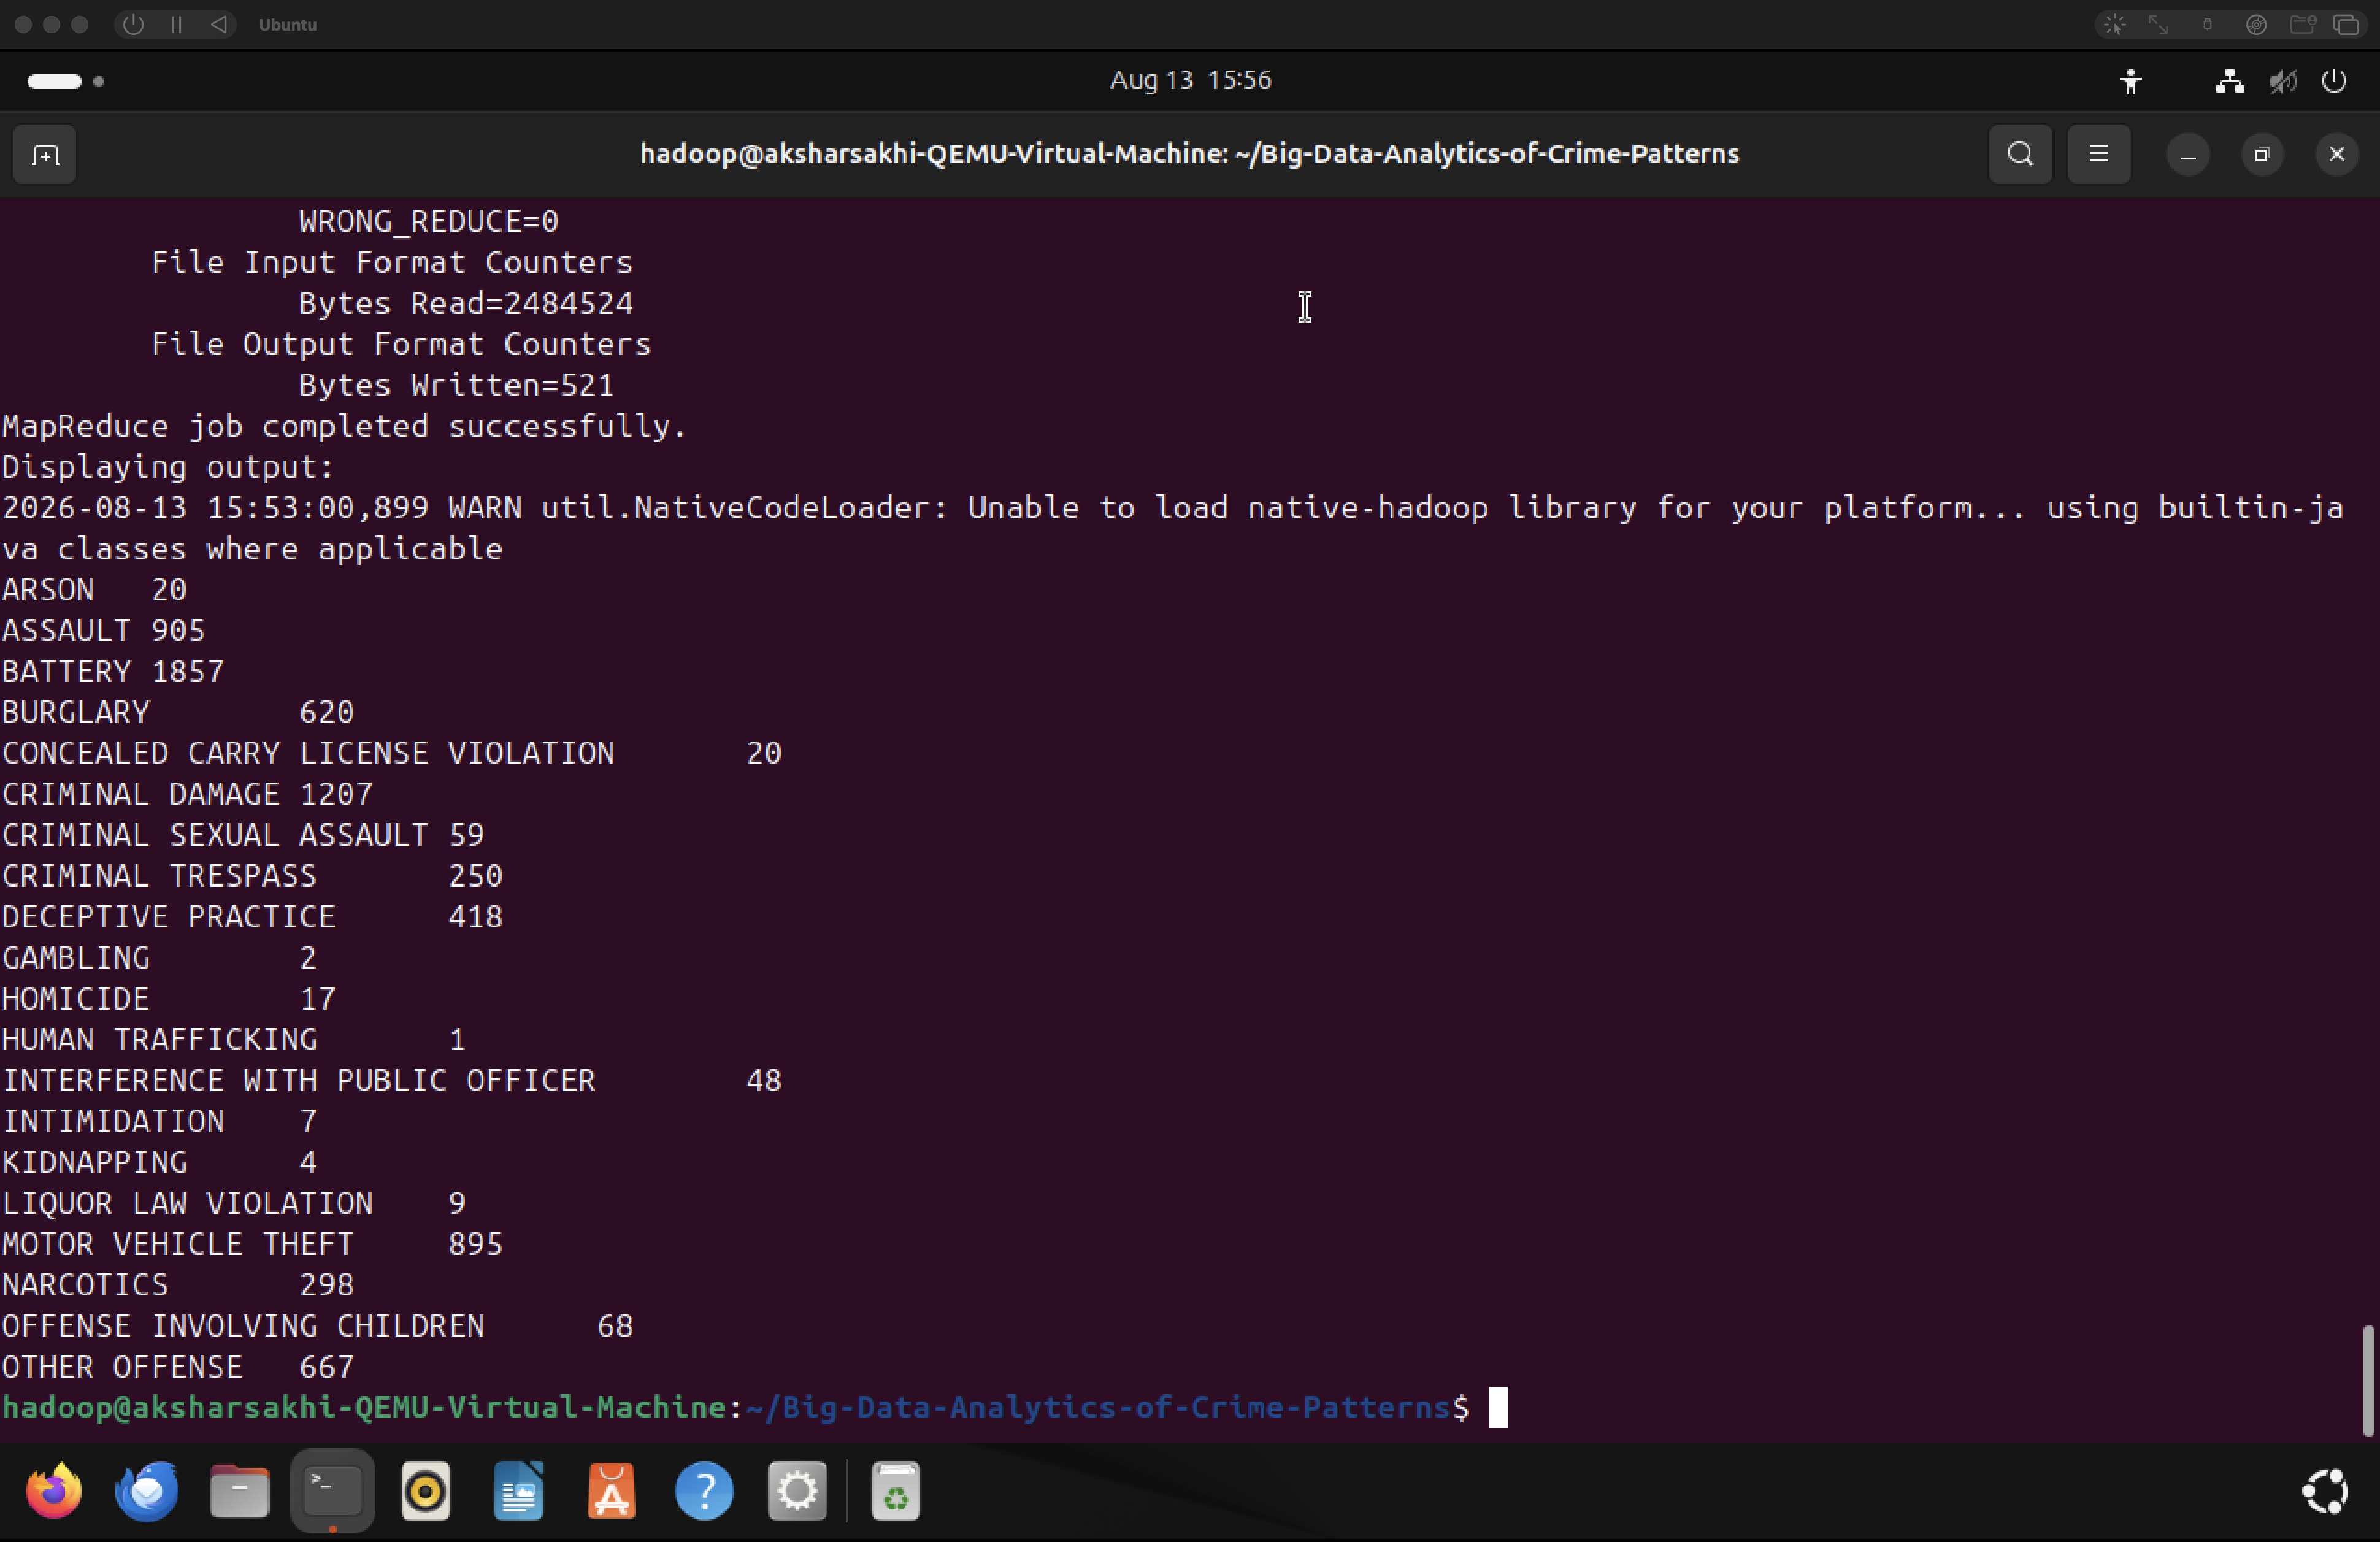
\includegraphics[width=0.8\textwidth]{images/mr_output.png}
    \caption{MapReduce Output showing crime counts.}
\end{figure}

\newpage
\section{Hive analysis questions}
The following 10 meaningful queries were executed in Apache Hive on the dataset to extract business intelligence. Table \ref{tab:hive_reqs} maps the rubric requirements to the implemented queries.

\begin{table}[h]
    \centering
    \begin{tabular}{@{}ll@{}}
        \toprule
        \textbf{Requirement} & \textbf{Query Implementation Focus} \\ \midrule
        SELECT & Retrieving basic incident records \\
        WHERE & Filtering specific crime types (Narcotics) and arrest statuses \\
        ORDER BY & Sorting homicides chronologically \\
        GROUP BY & Aggregating incidents by location description \\
        HAVING & Filtering for dominant crime categories (count $>$ 500) \\
        COUNT & Counting occurrences per category or location \\
        SUM & Calculating absolute total arrests per district \\
        AVG & Determining average domestic crime rates per beat \\
        MAX \& MIN & Pinpointing districts with highest and lowest crime volumes \\
        JOIN & Merging crimes with community area names for readability \\ \bottomrule
    \end{tabular}
    \caption{Mapping of Hive SQL Requirements to Queries}
    \label{tab:hive_reqs}
\end{table}

\section{Each query executions}

\textbf{1. SELECT - Retrieve the first 10 crime records.}
\begin{lstlisting}[language=SQL]
SELECT id, primary_type, description, crime_date
FROM crimes LIMIT 10;
\end{lstlisting}

\textbf{2. WHERE - Find all incidents where an arrest was made for narcotics.}
\begin{lstlisting}[language=SQL]
SELECT id, primary_type, description, arrest
FROM crimes WHERE primary_type = 'NARCOTICS' AND arrest = 'true' LIMIT 10;
\end{lstlisting}

\textbf{3. ORDER BY - List recent homicides ordered by date.}
\begin{lstlisting}[language=SQL]
SELECT case_number, primary_type, crime_date
FROM crimes WHERE primary_type = 'HOMICIDE'
ORDER BY crime_date DESC LIMIT 10;
\end{lstlisting}

\textbf{4. GROUP BY \& COUNT - Find the number of crimes per location description.}
\begin{lstlisting}[language=SQL]
SELECT location_description, COUNT(*) AS crime_count
FROM crimes GROUP BY location_description
ORDER BY crime_count DESC LIMIT 15;
\end{lstlisting}

\textbf{5. HAVING - Find primary crime types that occurred more than 500 times.}
\begin{lstlisting}[language=SQL]
SELECT primary_type, COUNT(*) as total
FROM crimes GROUP BY primary_type
HAVING COUNT(*) > 500 ORDER BY total DESC;
\end{lstlisting}

\textbf{6. SUM - Calculate the total number of arrests made per district.}
\begin{lstlisting}[language=SQL]
SELECT district, SUM(CASE WHEN arrest = 'true' THEN 1 ELSE 0 END) AS total_arrests
FROM crimes WHERE district IS NOT NULL AND district != ''
GROUP BY district ORDER BY total_arrests DESC LIMIT 10;
\end{lstlisting}

\textbf{7. AVG - Calculate the average number of domestic crimes per beat.}
\begin{lstlisting}[language=SQL]
SELECT beat, AVG(CASE WHEN domestic = 'true' THEN 1.0 ELSE 0.0 END) AS avg_domestic
FROM crimes WHERE beat IS NOT NULL AND beat != ''
GROUP BY beat ORDER BY avg_domestic DESC LIMIT 10;
\end{lstlisting}

\textbf{8. MAX - Find the district with the maximum reported cases.}
\begin{lstlisting}[language=SQL]
SELECT district, COUNT(*) AS district_total
FROM crimes WHERE district IS NOT NULL AND district != ''
GROUP BY district ORDER BY district_total DESC LIMIT 1;
\end{lstlisting}

\textbf{9. MIN - Find the district with the minimum reported cases.}
\begin{lstlisting}[language=SQL]
SELECT district, COUNT(*) AS district_total
FROM crimes WHERE district IS NOT NULL AND district != ''
GROUP BY district ORDER BY district_total ASC LIMIT 1;
\end{lstlisting}

\textbf{10. JOIN - Join crimes and community\_areas to display community names.}
\begin{lstlisting}[language=SQL]
SELECT c.case_number, c.primary_type, a.area_name
FROM crimes c JOIN community_areas a ON (c.community_area = a.area_code) LIMIT 15;
\end{lstlisting}

\section{Screenshot Query result}
\begin{figure}[h]
    \centering
    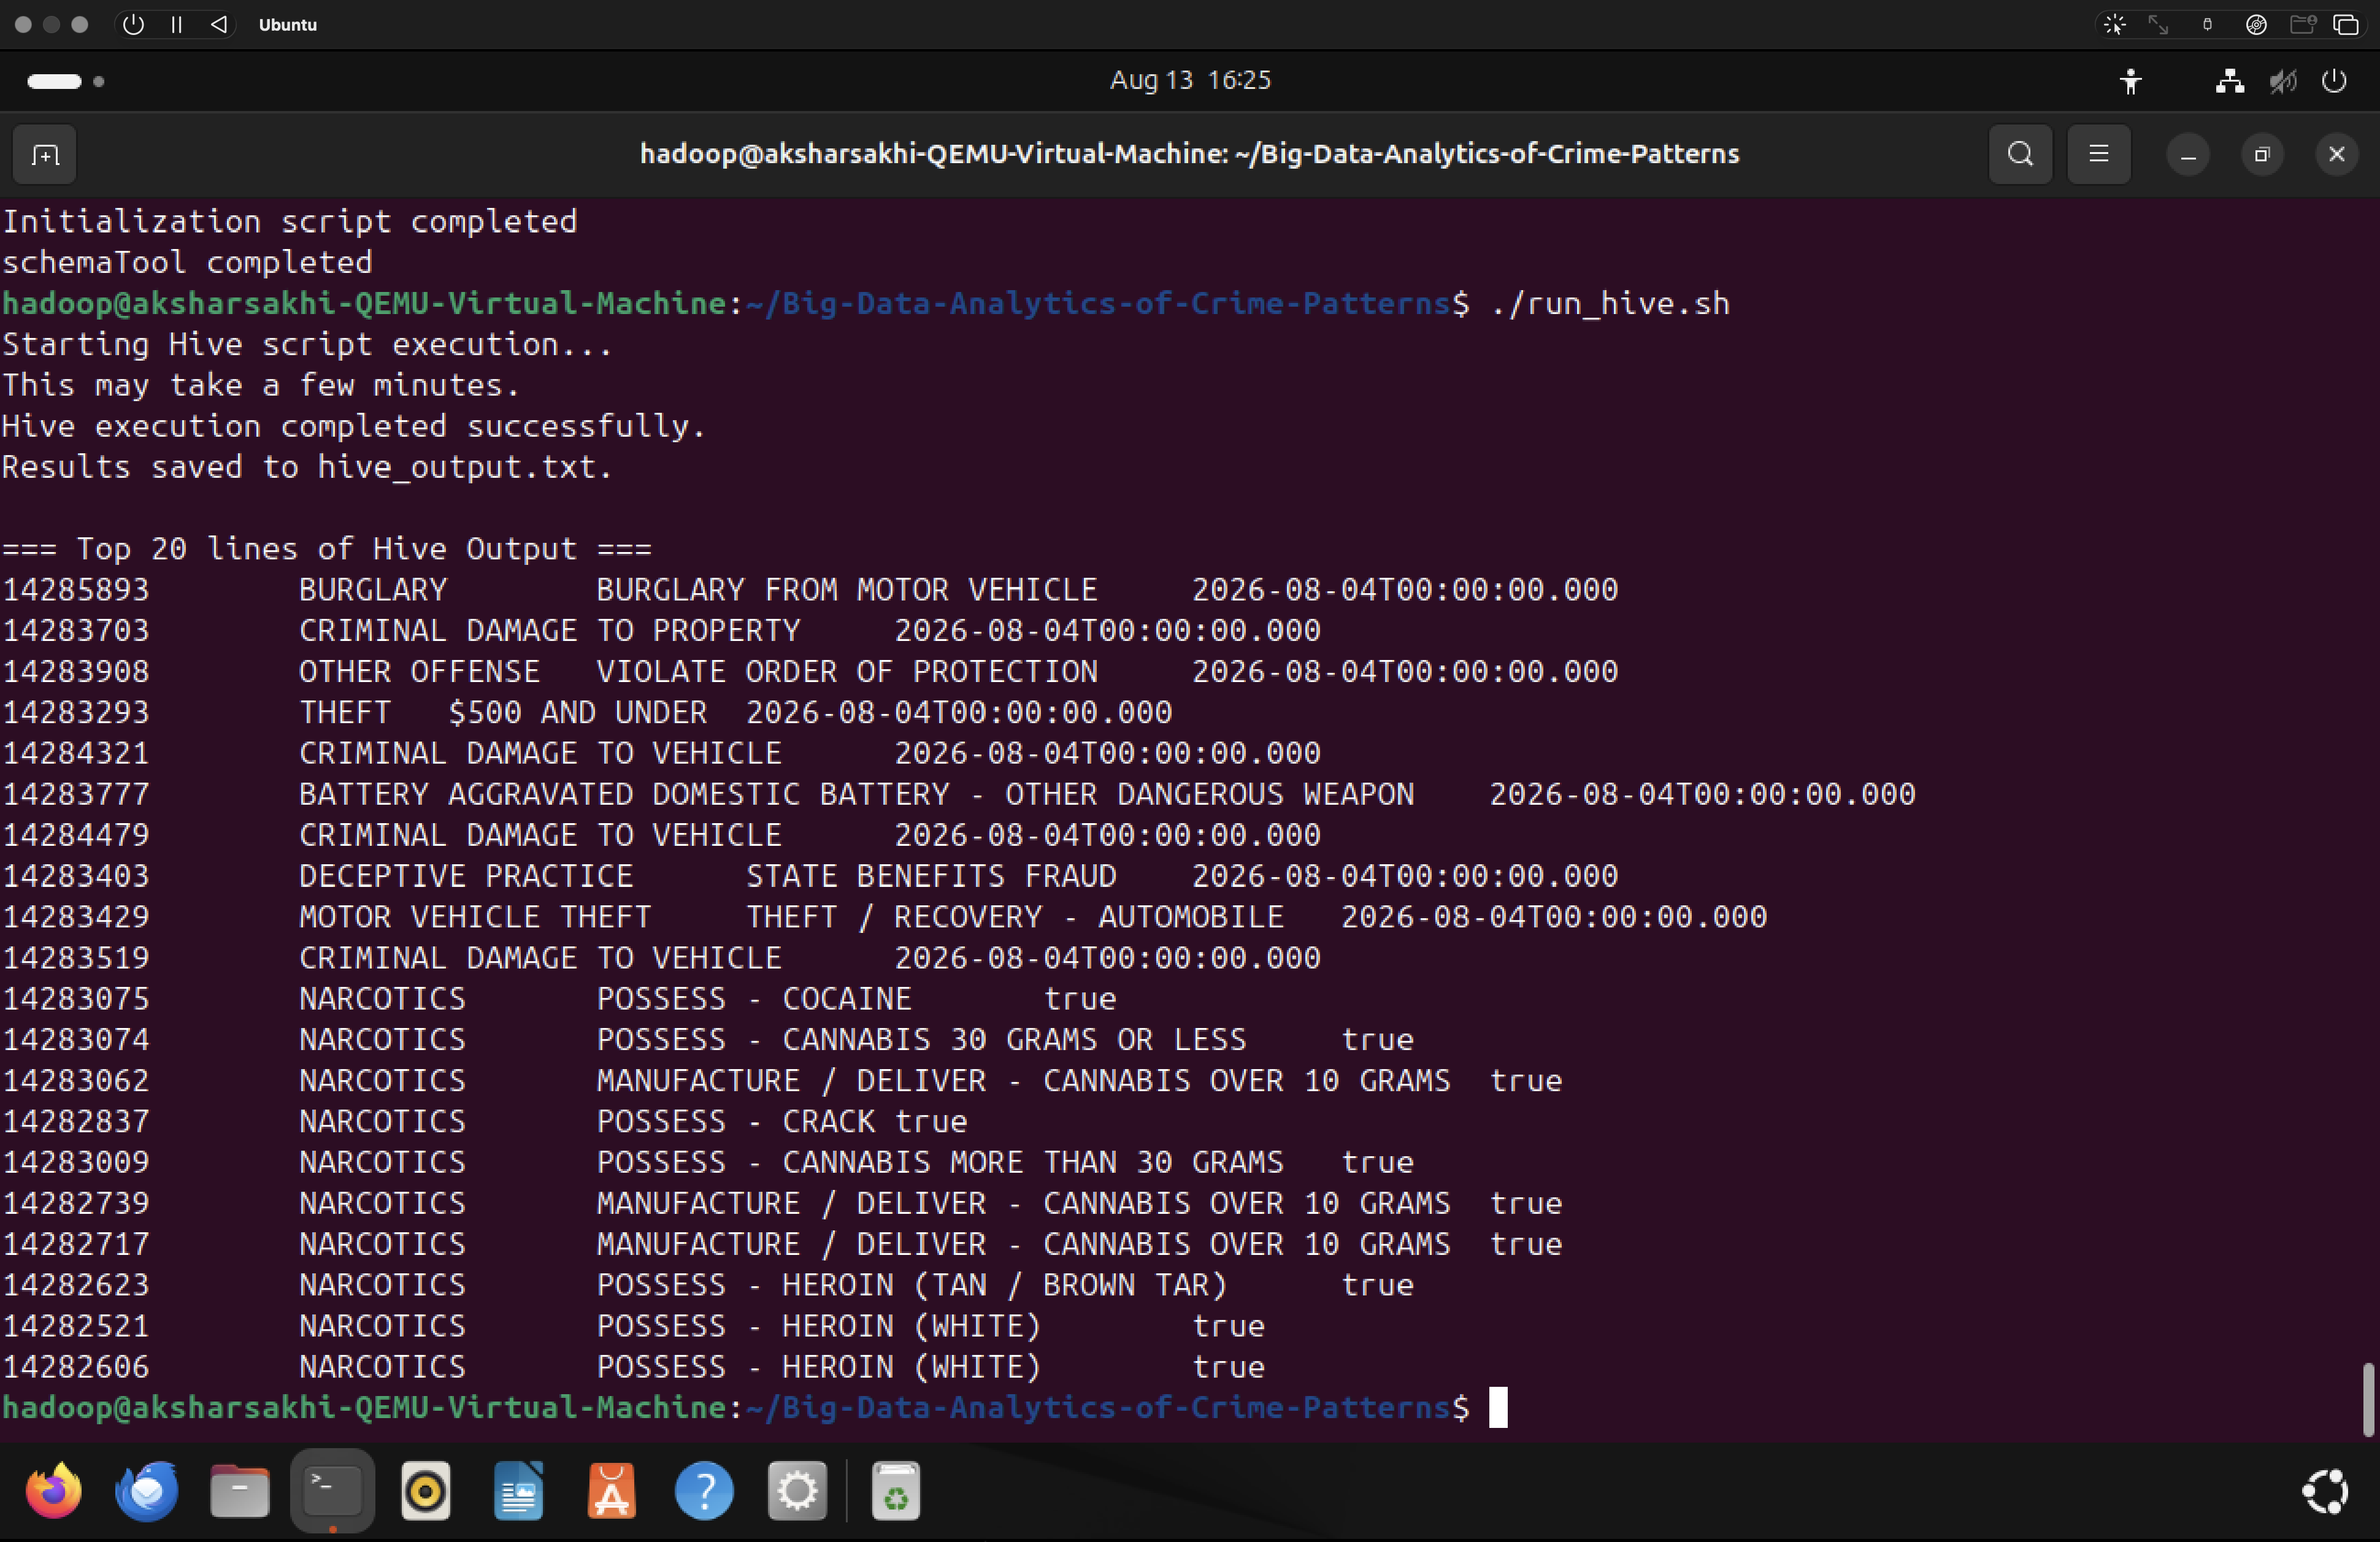
\includegraphics[width=0.8\textwidth]{images/hive_queries.png}
    \caption{Screenshots showing successful execution of Hive queries.}
\end{figure}

\section{Conclusion}
This project successfully demonstrated the end-to-end processing of a real-world Big Data application. Using the Chicago Crimes dataset, we successfully ingested data into HDFS, executed a Java MapReduce program to calculate crime type frequencies, and leveraged Apache Hive to perform advanced SQL-based analytical queries. The pipeline provides a scalable foundation for public safety data analysis.

\end{document}
